\documentclass{beamer}
\usetheme{Boadilla}
\usecolortheme{seahorse}
\usefonttheme{professionalfonts}
\usepackage{lmodern}

\usepackage{graphicx,xcolor}
\usepackage{amsmath,amssymb,amsfonts,bm}
\usepackage{booktabs,array,tabularx}
\usepackage{tikz}
\usetikzlibrary{arrows.meta,positioning,shapes.geometric,fit,calc}
\usepackage{hyperref}

\setbeamertemplate{caption}[numbered]
\setbeamertemplate{navigation symbols}{}
\setbeamertemplate{title page}[default]
\graphicspath{{images/}{images/eda/}{images/modwt/}{images/results/}{images/paper/}{images/logo/}{images/illustrate/}}

\title[WaveCatBoost]{WaveCatBoost: Hybrid Air Quality Forecasting}
\subtitle{Applied Time Series Analysis --- Course Project\\[0.4em]\textbf{Group 8}}
\author[Group 8]{%
  Kumar Utkarsh \and
  M~Charan Sree Teja \and
  P~Sai Deva Charan \and
  D~Lalit Santosh%
}
\institute[MFSDS\&AI]{Mehta Family School of Data Science and Artificial Intelligence}
\date{\today}

\begin{document}

\begin{frame}
  \titlepage
\end{frame}

\section{Problem and Approach}
\begin{frame}{Problem and Approach}
  \begin{block}{Why this is hard}
    \begin{itemize}
      \item Air-quality forecasting needs \textbf{near real-time} answers.
      \item That pushes us toward \textbf{lighter} models (trees, short lags).
      \item The series is \textbf{non-stationary}: spikes, regime shifts, and changing variance.
      \item Light models struggle on the \textbf{raw} mix of spikes, diurnal cycles, and slow drift.
    \end{itemize}
  \end{block}

  \begin{exampleblock}{Paper approach}
    \begin{enumerate}
      \item Split the series into scale-wise components (details + smooth) with Haar MODWT.
      \item Forecast each component with CatBoost.
      \item Reconstruct by summing bands; optionally add conformal intervals.
    \end{enumerate}
  \end{exampleblock}
\end{frame}


\section{Datasets and Preprocessing}
\begin{frame}{Datasets}
  \begin{columns}[T]
    \begin{column}{0.38\textwidth}
      {\footnotesize
      \textbf{Paper CSVs (Meghalaya, hourly)}
      \begin{itemize}\setlength\itemsep{0.15em}
        \item \textbf{CPCB}, \textbf{ID1} from Borah et al.
        \item $n \approx 8880$ / $9505$.
        \item NO$_2$, O$_3$, CO, SO$_2$, PM$_{2.5}$, PM$_{10}$.
      \end{itemize}
      \textbf{Extra CAAQMS (15-min $\to$ hourly)}
      \begin{itemize}\setlength\itemsep{0.15em}
        \item \textbf{Shillong:} Lumpyngngad, JN Stadium.
        \item Delhi: ITO, R~K~Puram.
      \end{itemize}
      }
    \end{column}
    \begin{column}{0.60\textwidth}
      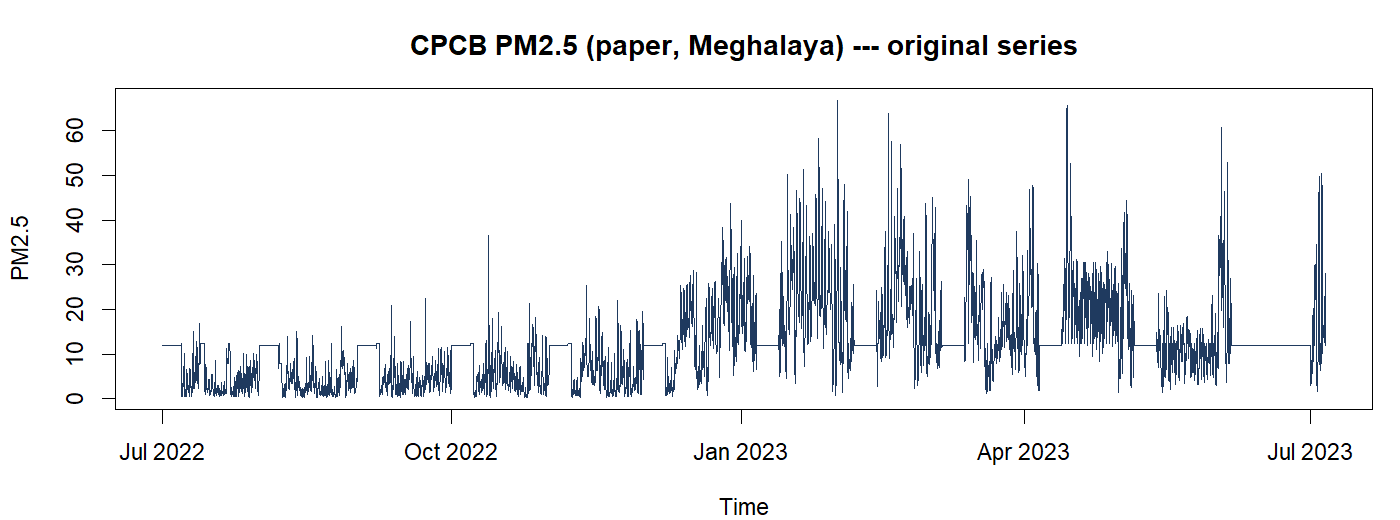
\includegraphics[width=\linewidth]{series_cpcb_pm25.png}\\[-0.2em]
      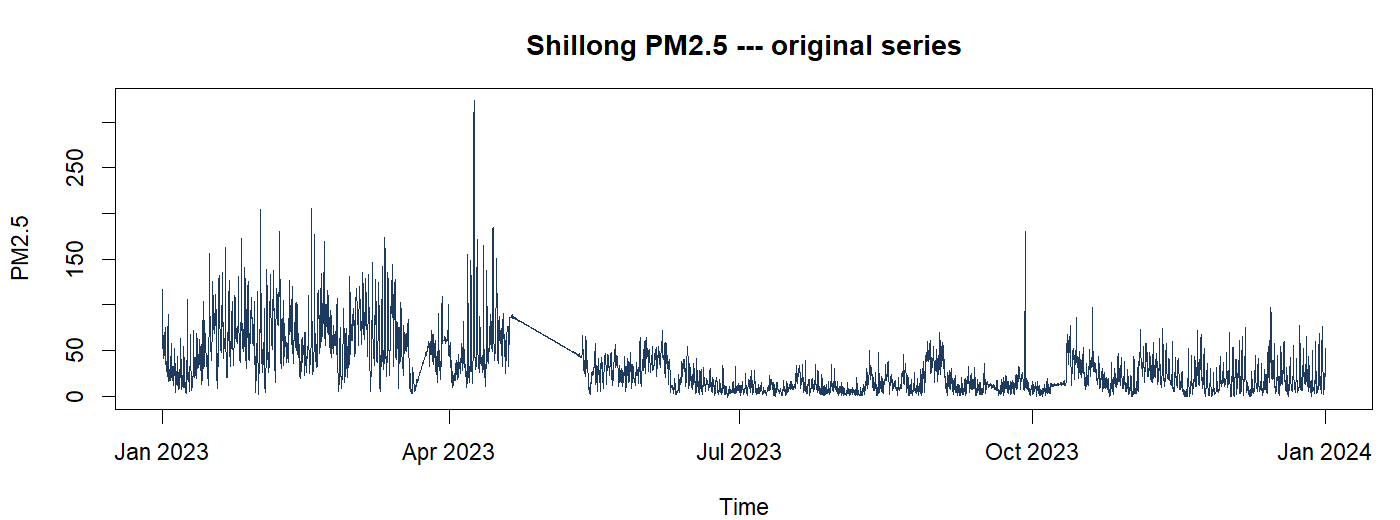
\includegraphics[width=\linewidth]{series_shillong_pm25.png}
    \end{column}
  \end{columns}
\end{frame}

\begin{frame}{Dataset diagnostics --- CPCB PM$_{2.5}$}
  \centering
  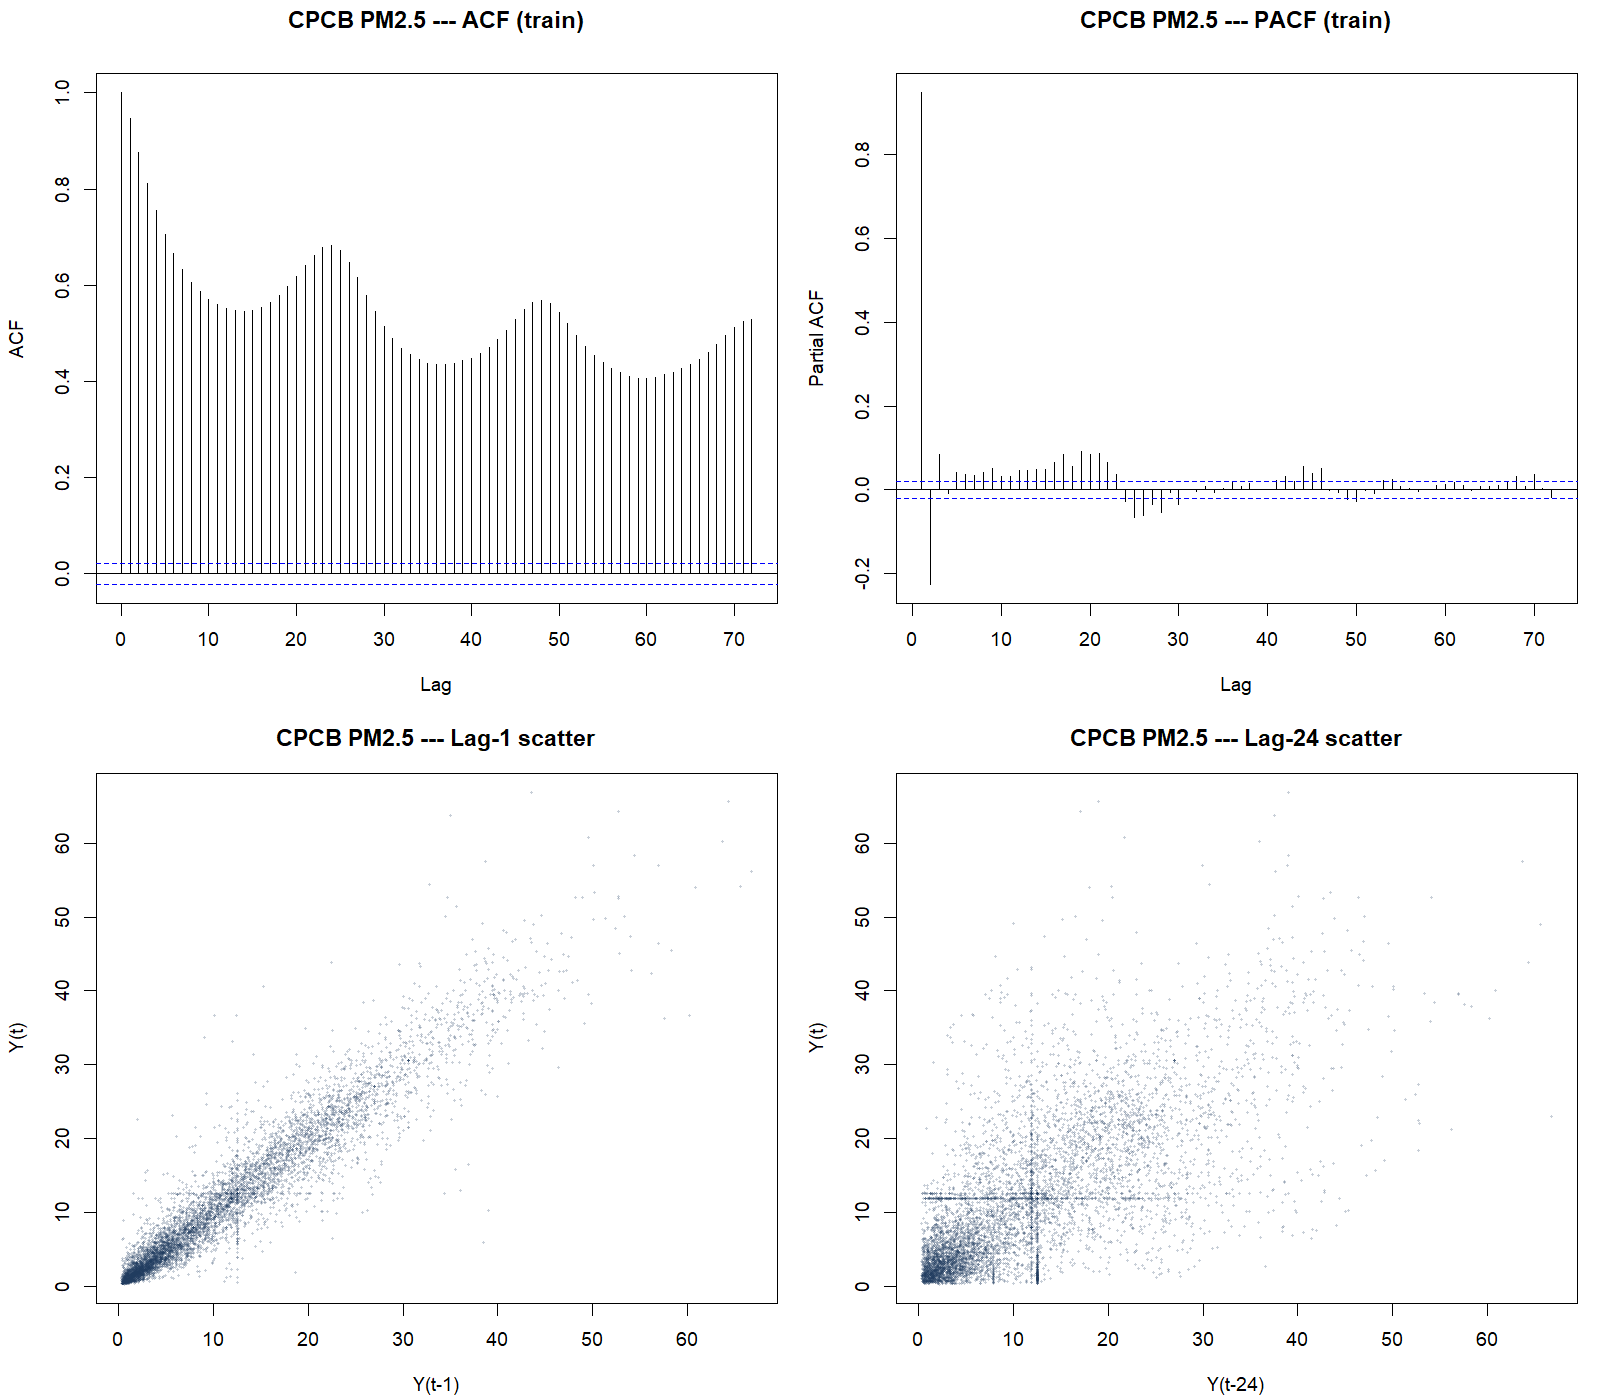
\includegraphics[width=0.98\linewidth,height=0.82\textheight,keepaspectratio]{diag_2x2_cpcb_pm25.png}
\end{frame}

\begin{frame}{Seasonal structure --- CPCB PM$_{2.5}$}
  \centering
  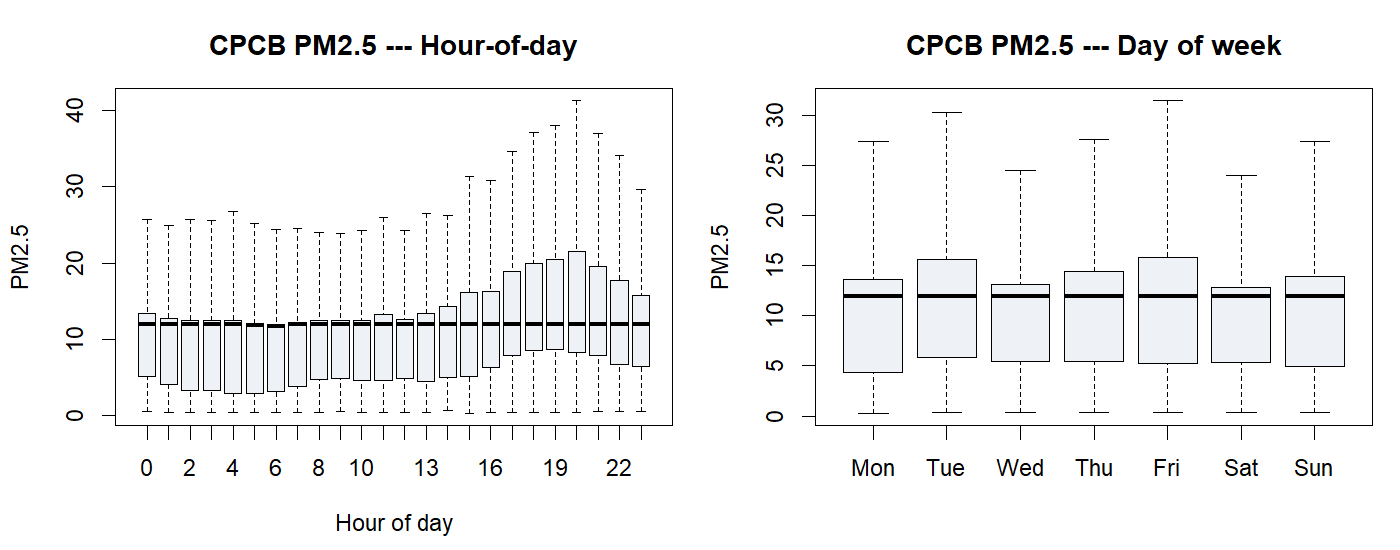
\includegraphics[width=0.95\linewidth,height=0.70\textheight,keepaspectratio]{boxes_cpcb_pm25.png}
  \vspace{0.15em}
  \begin{itemize}
    \item Clear diurnal pattern; milder weekday effect.
    \item Motivates $S=24$ baselines and lag features up to 24~h.
  \end{itemize}
\end{frame}

\begin{frame}{What we did before modelling}
  \begin{itemize}
    \item \textbf{Hourly grid:} end-labelled hourly means (15-min CAAQMS $\to$ hour $t$).
    \item \textbf{Quality screen:} physical bounds, stuck sensors, spike flags.
    \item \textbf{Causal fill:} impute only with information available up to the cut time.
    \item \textbf{Chronological split:} train $\to$ val (tuning) $\to$ test (last $h$ hours).\\
          Horizons $h\in\{24,168,336,744\}$.
    \item \textbf{Scale:} min--max to $[0,1]$ fit on \textbf{train only}.
    \item Paper Meghalaya CSVs are already hourly $\Rightarrow$ skip re-aggregation / fill.\\
          Extra stations (Shillong, Delhi) get the full clean path into an isolated store.
  \end{itemize}
\end{frame}


\section{MODWT Decomposition}
\begin{frame}{Why decompose? Why not Fourier?}
  \begin{block}{Why split the series}
    \begin{itemize}
      \item Raw $Y_t$ mixes noise, diurnal swings, and slow level shifts.
      \item One light model on the mix misses scale-specific structure.
      \item Decompose $\to$ forecast each band $\to$ add back $=$ richer dynamics without a heavy global model.
    \end{itemize}
  \end{block}
  \begin{alertblock}{Why not Fourier}
    \begin{itemize}
      \item Fourier uses \textbf{global} sinusoids over the whole record.
      \item Air quality is \textbf{non-stationary} --- spikes and regime changes are local in time.
      \item Wavelets give a joint \textbf{time--scale} view; MODWT keeps every band length $N$ (no downsampling).
      \item Haar MRA is additive: $Y_t=\sum_k D_{k,t}+S_{K,t}$.
    \end{itemize}
  \end{alertblock}
\end{frame}

\begin{frame}{MODWT: additive components}
  \begin{columns}[T]
    \begin{column}{0.40\textwidth}
      \[
        Y_t = \sum_{k=1}^{K} D_{k,t} + S_{K,t}
      \]
      {\footnotesize
      \begin{itemize}
        \item $D_{k,t}$: detail at scale $\sim 2^{k}$~h.
        \item $S_{K,t}$: smooth after $K$ levels.
        \item Paper: $K\approx\ln N$; we use $K{=}4$--$5$ ($\sim 16$--$32$~h smooth).
        \item $D_1$: high-frequency component;\\
              $D_k$: lower-frequency component;\\
              $S_K$: smooth trend / level.
      \end{itemize}
      }
    \end{column}
    \begin{column}{0.58\textwidth}
      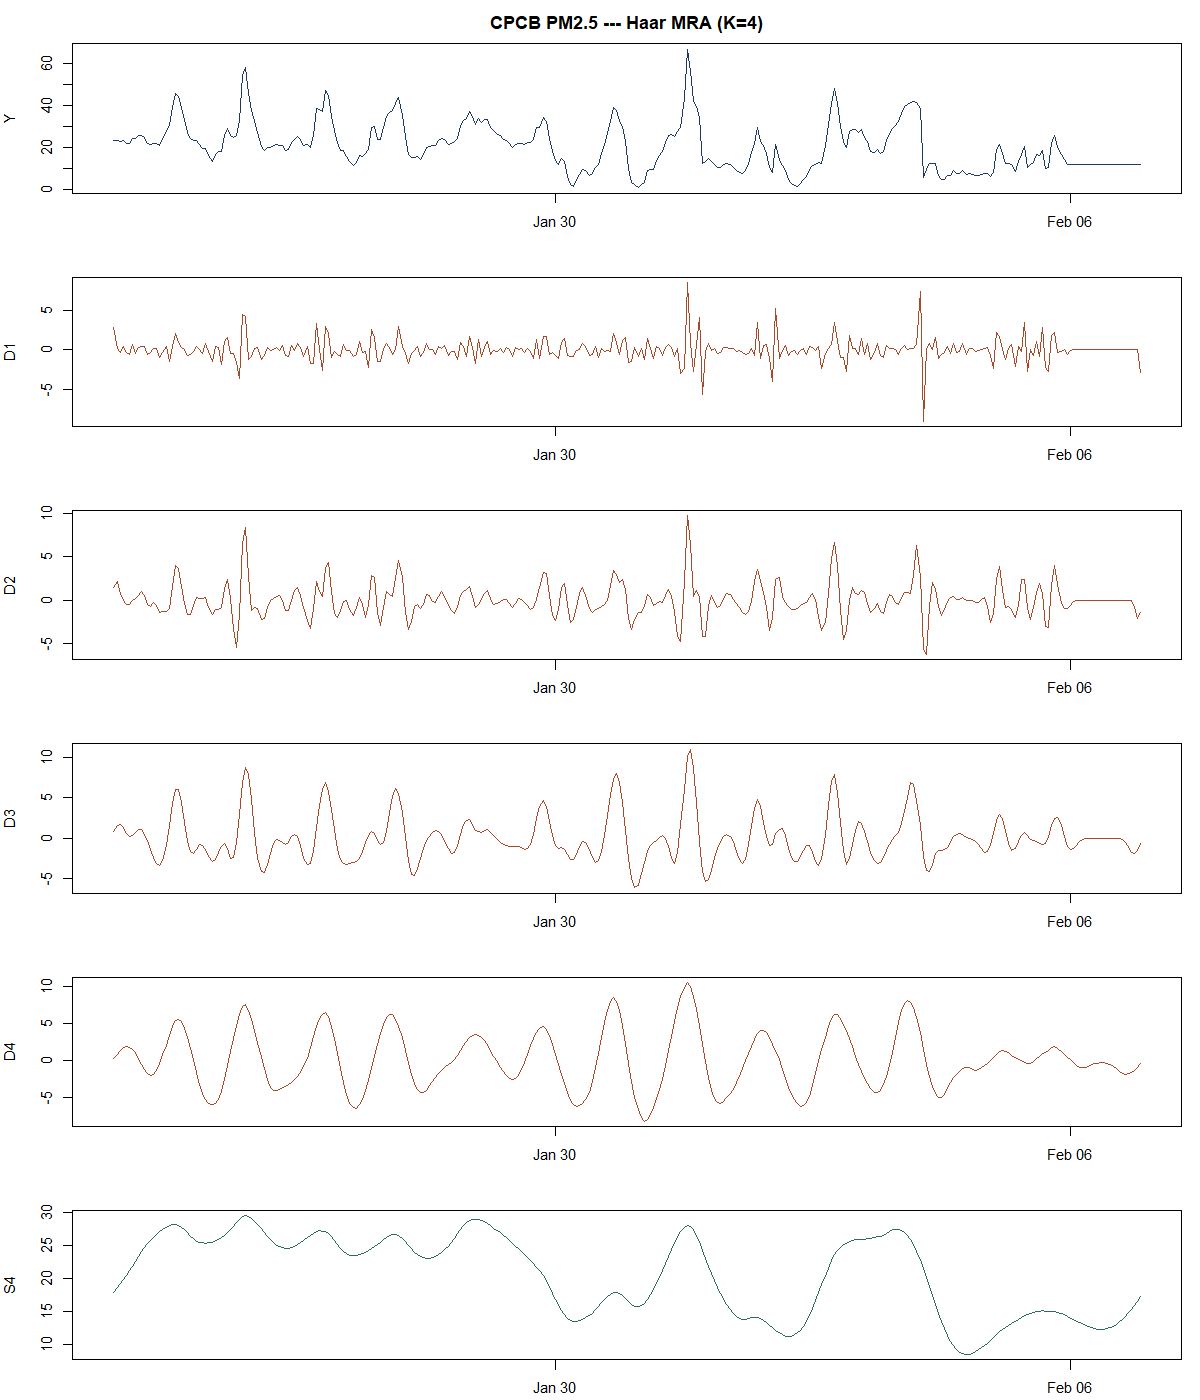
\includegraphics[width=\linewidth,height=0.78\textheight,keepaspectratio]{mra_d1d4_s4_cpcb_pm25.png}
    \end{column}
  \end{columns}
\end{frame}

% Mathematical intuition --- boxed filters like reference slide; compact tree
\begin{frame}{MODWT: mathematical intuition}
  \begin{columns}[T]
    \begin{column}{0.50\textwidth}
      {\scriptsize
      \noindent
      \fcolorbox{gray!55}{gray!12}{\parbox{0.96\linewidth}{%
        \textbf{Wavelet filter:} $p_m\to D$ (details)\\
        $\sum_m p_m=0$ \ (measures change)}}\\[0.3em]
      \fcolorbox{gray!55}{gray!12}{\parbox{0.96\linewidth}{%
        \textbf{Scaling filter:} $q_m\to S$ (smooth)\\
        $\sum_m q_m=1$ \ (measures average)}}\\[0.4em]
      \textbf{Filter condition} (nonzero $n$):\\
      $\sum_m p_m p_{m+2n}=\sum_m q_m q_{m+2n}=0$\\[0.35em]
      \textbf{Recursion at level $j$}\ ($S_{0,t}=Y_t$)\\[0.15em]
      $D_{j,t}=\sum_{m}p_m\,S_{j-1,(t-2^{j-1}m)\bmod N}$\\[0.1em]
      $S_{j,t}=\sum_{m}q_m\,S_{j-1,(t-2^{j-1}m)\bmod N}$\\[0.25em]
      Haar: $q=(\tfrac12,\tfrac12)$,\ $p=(\tfrac12,-\tfrac12)$.\\
      Tap spacing doubles each level.
      }
    \end{column}
    \begin{column}{0.48\textwidth}
      \centering
      \resizebox{0.88\linewidth}{!}{%
      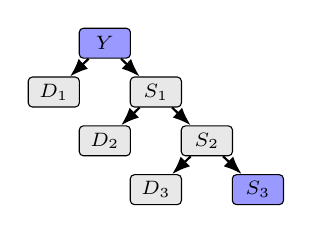
\begin{tikzpicture}[
        font=\scriptsize,
        x=0.72cm, y=0.62cm,
        box/.style={draw, rounded corners=1.5pt, align=center,
                    inner sep=1.2pt, minimum width=0.65cm, minimum height=0.38cm},
        ybox/.style={box, fill=blue!40},
        dbox/.style={box, fill=gray!18},
        sbox/.style={box, fill=gray!18},
        arr/.style={-{Latex}, thick}
      ]
        \node[ybox] (y)  at (0.9, 0) {$Y$};
        \node[dbox] (d1) at (0.0,-1.0) {$D_1$};
        \node[sbox] (s1) at (1.8,-1.0) {$S_1$};
        \node[dbox] (d2) at (0.9,-2.0) {$D_2$};
        \node[sbox] (s2) at (2.7,-2.0) {$S_2$};
        \node[dbox] (d3) at (1.8,-3.0) {$D_3$};
        \node[ybox] (s3) at (3.6,-3.0) {$S_3$};
        \draw[arr] (y)  -- (d1);
        \draw[arr] (y)  -- (s1);
        \draw[arr] (s1) -- (d2);
        \draw[arr] (s1) -- (s2);
        \draw[arr] (s2) -- (d3);
        \draw[arr] (s2) -- (s3);
      \end{tikzpicture}%
      }

      \vspace{0.2em}
      {\scriptsize
      Only the smooth is split again.\\
      $Y=D_1+D_2+D_3+S_3$\\[0.25em]
      \textbf{Inverse (IMODWT):} same filters, reversed\\
      \resizebox{\linewidth}{!}{$
        S_{j-1,t}=\sum_m p_m D_{j,t+2^{j-1}m}
        +\sum_m q_m S_{j,t+2^{j-1}m}
      $}
      }
    \end{column}
  \end{columns}
\end{frame}

\begin{frame}{Filter coefficients}
  \centering
  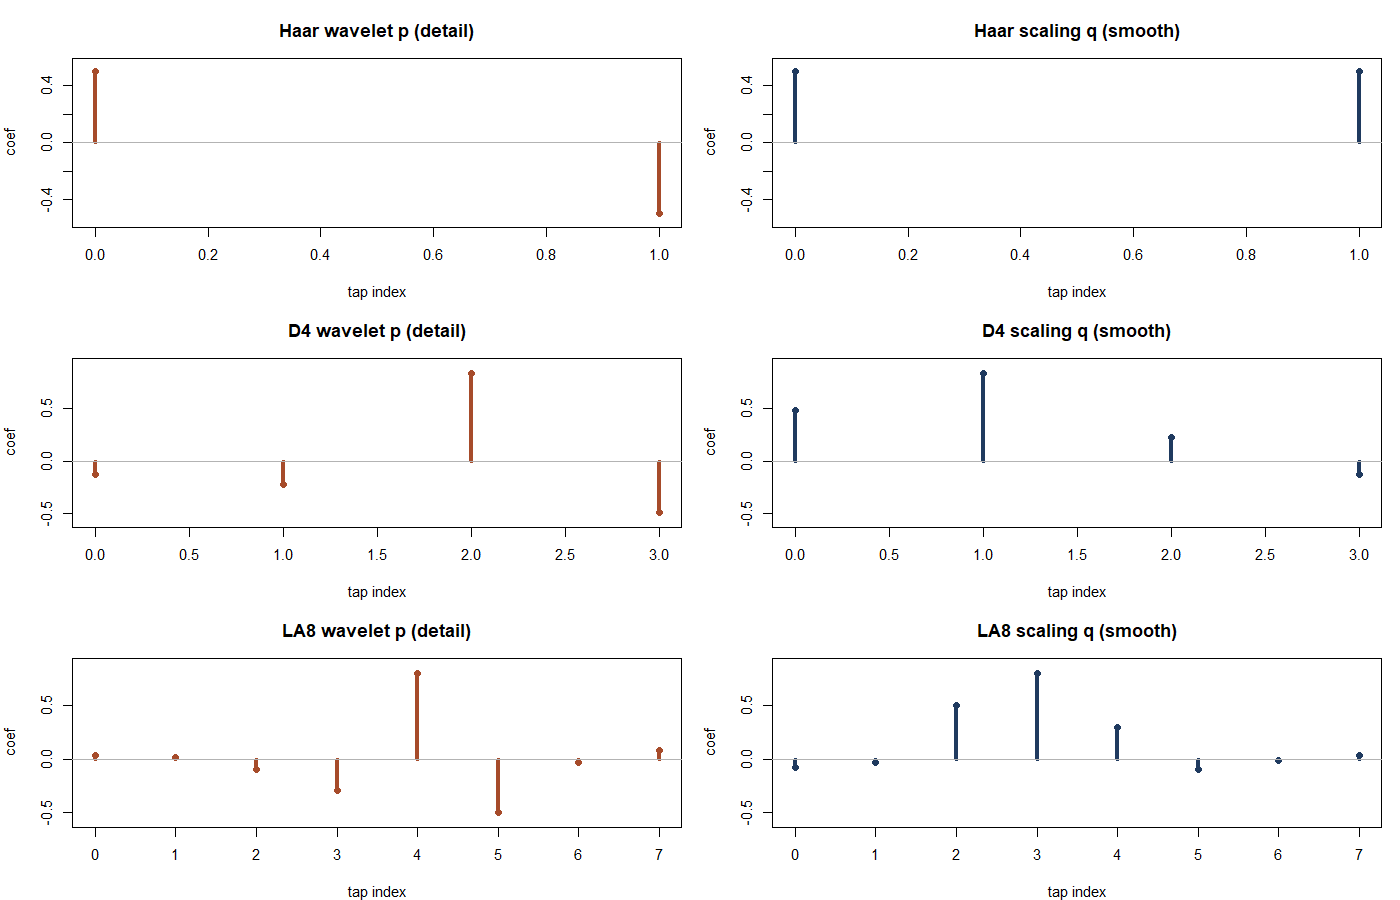
\includegraphics[width=0.95\linewidth,height=0.78\textheight,keepaspectratio]{filter_taps.png}
\end{frame}

\begin{frame}{Haar vs D4 vs LA8 (WaveCatBoost, 1-day MASE)}
  \begin{itemize}\setlength\itemsep{0.2em}
    \item \textbf{Paper default:} Haar ($M{=}2$).
    \item \textbf{We also tried:} D4 ($M{=}4$) and LA8 ($M{=}8$).
    \item Same WaveCatBoost head, same $K$ and lag $p$.
  \end{itemize}
  \vspace{0.4em}
  \centering
  \begin{tabular}{llccc}
    \toprule
    Sensor & Pollutant & Haar & D4 & LA8 \\
    \midrule
    CPCB & NO$_2$    & 0.541 & 0.510 & 0.529 \\
    CPCB & PM$_{2.5}$ & 0.727 & 0.909 & 0.955 \\
    ID1  & NO$_2$    & 1.252 & 1.346 & 1.330 \\
    ID1  & PM$_{2.5}$ & 0.421 & 0.457 & 0.502 \\
    \bottomrule
  \end{tabular}
  \vspace{0.5em}
  \begin{exampleblock}{Takeaway}
    Haar wins on 3 of 4 cells (D4 edges CPCB NO$_2$). Longer filters do not help overall --- Haar stays the default.
  \end{exampleblock}
\end{frame}


\section{CatBoost and Conformal Prediction}
% WaveCatBoost methodology + conformal prediction

\begin{frame}{WaveCatBoost pipeline}
  \centering
  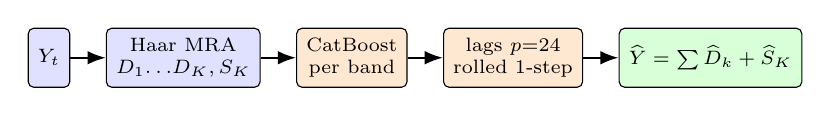
\begin{tikzpicture}[
    font=\scriptsize,
    box/.style={draw, rounded corners=2pt, align=center, inner sep=3.5pt, minimum height=0.75cm},
    arr/.style={-{Latex}, thick}
  ]
    \node[box, fill=blue!12] (y) {$Y_t$};
    \node[box, fill=blue!12, right=0.45cm of y] (mra) {Haar MRA\\$D_1{\ldots}D_K,S_K$};
    \node[box, fill=orange!18, right=0.45cm of mra] (cb) {CatBoost\\per band};
    \node[box, fill=orange!18, right=0.45cm of cb] (rec) {lags $p{=}24$\\rolled 1-step};
    \node[box, fill=green!15, right=0.45cm of rec] (inv) {$\widehat Y=\sum \widehat D_k+\widehat S_K$};

    \draw[arr] (y) -- (mra);
    \draw[arr] (mra) -- (cb);
    \draw[arr] (cb) -- (rec);
    \draw[arr] (rec) -- (inv);
  \end{tikzpicture}

  \vspace{0.55em}
  {\footnotesize
  \begin{itemize}\setlength\itemsep{0.35em}
    \item Paper hybrid (Borah et al.): decompose $\to$ light tree per scale $\to$ sum.
    \item Same $K$ and lag $p$ for every Wave\* head; only the tree family changes.
    \item Point forecast alone is not enough for air-quality decisions --- we need uncertainty
          (next slides).
  \end{itemize}
  }
\end{frame}

\begin{frame}{Why CatBoost on each band?}
  \begin{columns}[T]
    \begin{column}{0.52\textwidth}
      \begin{block}{Why a tree head}
        {\footnotesize
        \begin{itemize}\setlength\itemsep{0.3em}
          \item Fast enough for near real-time AQ use.
          \item Handles nonlinear lag effects without a deep net.
          \item CatBoost: ordered boosting, strong default regularisation.
          \item Paper picks CatBoost over raw LGB / XGB / RNNs on MASE.
        \end{itemize}
        }
      \end{block}
    \end{column}
    \begin{column}{0.46\textwidth}
      \begin{block}{Why \emph{one model per band}}
        {\footnotesize
        \begin{itemize}\setlength\itemsep{0.3em}
          \item $D_1$: spiky, high-frequency noise.
          \item $D_k$: mid-scale diurnal swings.
          \item $S_K$: slow level / trend.
          \item Separate CatBoosts learn band-specific lag structure;
                a single raw model mixes all scales.
        \end{itemize}
        }
      \end{block}
    \end{column}
  \end{columns}
  \vspace{0.45em}
  \begin{exampleblock}{Family}
    WaveCatBoost $=$ Haar MRA $+$ CatBoost$(D_1),\ldots,$CatBoost$(S_K)$.\\
    WaveLGB / WaveXGB keep the same bands; only the fitter changes.
  \end{exampleblock}
\end{frame}

\begin{frame}{Features, rolled forecast, reconstruct}
  {\footnotesize
  \textbf{Features (each band).} Lag vector of length $p$:
  \[
    \mathbf{x}_t^{(k)}
    =\big(D_{k,t-1},\ldots,D_{k,t-p}\big)
    \quad\text{(same for $S_K$)}.
  \]
  No calendar / weather covariates in the letter WaveCatBoost head.
  }
  \vspace{0.25em}
  \begin{columns}[T]
    \begin{column}{0.48\textwidth}
      \begin{block}{Rolled 1-step ($h$ origins)}
        {\footnotesize
        For each test hour $t$:
        \begin{enumerate}\setlength\itemsep{0.2em}
          \item Build lag row from \emph{observed} history.
          \item Predict one step with CatBoost.
          \item Append the true $Y_t$; advance the origin.
        \end{enumerate}
        Bake-off protocol in \texttt{scores.csv}
        (teacher forcing / walk-forward).
        }
      \end{block}
    \end{column}
    \begin{column}{0.50\textwidth}
      \begin{block}{Reconstruct}
        {\footnotesize
        Additive MRA $\Rightarrow$ just sum:
        \[
          \widehat Y_{t}
          =\sum_{k=1}^{K}\widehat D_{k,t}
           +\widehat S_{K,t}.
        \]
        Equivalent to IMODWT when bands are
        Haar MRA details $+$ smooth.\\[0.25em]
        Same rolled idea as the letter notebook;
        we recompute MRA on the growing prefix
        (no test leakage into train filters).
        }
      \end{block}
    \end{column}
  \end{columns}
\end{frame}

\begin{frame}{WaveCatBoost hyperparameters}
  {\footnotesize
  Paper does not publish tree settings. We screen once on \textbf{CPCB PM$_{2.5}$}
  (train only, 1-day split) and freeze for every sensor / pollutant.
  }
  \vspace{0.35em}
  \centering
  {\footnotesize
  \begin{tabular}{lc}
    \toprule
    Setting & Frozen value \\
    \midrule
    Wavelet filter & Haar \\
    Depth $K$ ($J$) & 5 (capped; WaveLGB CV preferred 9) \\
    Lag $p$ & 24 \\
    Tree depth & 6 \\
    Learning rate $\eta$ & 0.05 \\
    Rounds / early stop & 160 / 30 \\
    \bottomrule
  \end{tabular}
  }
  \vspace{0.45em}
  \begin{itemize}\setlength\itemsep{0.25em}
    \item Screening grid uses \textbf{LightGBM as a fast proxy}; winning
          $(p,\text{depth},\eta,K)$ reused by WaveCatBoost.
    \item Letter-notebook run: CatBoost, lags 24, 1000 trees
          (same rolled idea; separate cache).
  \end{itemize}
\end{frame}

\begin{frame}{WaveCatBoost --- training sketch}
  \centering
  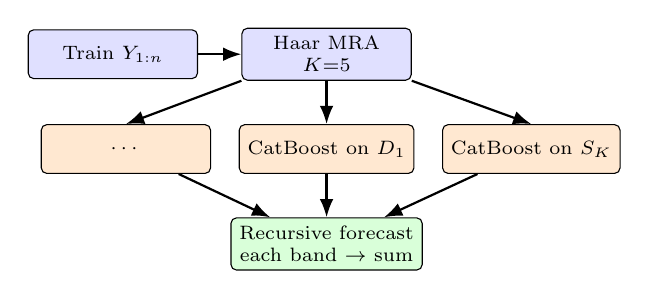
\begin{tikzpicture}[
    font=\scriptsize,
    box/.style={draw, rounded corners=2pt, align=center, inner sep=3pt,
                minimum width=2.15cm, minimum height=0.62cm},
    arr/.style={-{Latex}, thick}
  ]
    \node[box, fill=blue!12] (train) {Train $Y_{1:n}$};
    \node[box, fill=blue!12, right=0.55cm of train] (mra) {Haar MRA\\$K{=}5$};
    \node[box, fill=orange!18, below=0.55cm of mra] (d1) {CatBoost on $D_1$};
    \node[box, fill=orange!18, left=0.35cm of d1] (d2) {$\cdots$};
    \node[box, fill=orange!18, right=0.35cm of d1] (sk) {CatBoost on $S_K$};
    \node[box, fill=green!15, below=0.55cm of d1] (fc) {Recursive forecast\\each band $\to$ sum};

    \draw[arr] (train) -- (mra);
    \draw[arr] (mra) -- (d1);
    \draw[arr] (mra.south west) -- (d2.north);
    \draw[arr] (mra.south east) -- (sk.north);
    \draw[arr] (d1) -- (fc);
    \draw[arr] (d2) -- (fc);
    \draw[arr] (sk) -- (fc);
  \end{tikzpicture}

  \vspace{0.55em}
  {\footnotesize
  \begin{itemize}\setlength\itemsep{0.3em}
    \item Fit CatBoosts on \textbf{train bands only}; scaler also fit on train.
    \item Val (14\,d) used only for the one-time hyperparameter screen.
    \item Test $=$ last $h$ hours; score MASE / MAE / RMSE after inverse scaling.
  \end{itemize}
  }
\end{frame}

% ---- Metrics + bake-off (before conformal) ----
\begin{frame}{Error metrics (formulas)}
  {\footnotesize
  With train length $N$, horizon $h$, seasonality $S{=}24$:
  \[
    \mathrm{MASE}
    =\frac{\tfrac1h\sum_{t=1}^{h}|\widehat Y_t-Y_t|}
          {\tfrac1{N-S}\sum_{t=S+1}^{N}|Y_t-Y_{t-S}|}
  \]
  (equivalent to paper Eq.~(6) / Hyndman seasonal MASE).\\[0.4em]
  \[
    \mathrm{MAE}=\tfrac1h\sum_{t=1}^{h}|\widehat Y_t-Y_t|,
    \qquad
    \mathrm{RMSE}=\sqrt{\tfrac1h\sum_{t=1}^{h}(\widehat Y_t-Y_t)^2}.
  \]
  }
  \vspace{0.3em}
  \begin{itemize}
    \item MASE $<1$: better than seasonal naive on the train scale.
    \item Lower is better for all three.
  \end{itemize}
\end{frame}



\begin{frame}{MASE by horizon --- CPCB and ID1}
  \centering
  {\fontsize{5.6}{6.2}\selectfont
  \setlength{\tabcolsep}{3.5pt}
  \begin{tabular}{llcccc|cccc}
    \toprule
    & & \multicolumn{4}{c|}{CPCB} & \multicolumn{4}{c}{ID1} \\
    Pol. & $h$ & snaive & LGB & CatBoost & WaveCB & snaive & LGB & CatBoost & WaveCB \\
    \midrule
    \multirow{4}{*}{PM$_{2.5}$} & 1d & 2.02 & 0.74 & 0.82 & \textbf{0.65} & 0.71 & 0.84 & 0.67 & \textbf{0.42} \\
     & 7d & 2.32 & 0.81 & 0.90 & \textbf{0.71} & 0.82 & 0.93 & 0.74 & \textbf{0.65} \\
     & 14d & 2.63 & 0.87 & 0.97 & \textbf{0.77} & 0.92 & 1.00 & 0.79 & \textbf{0.70} \\
     & 31d & 2.93 & 0.94 & 1.04 & \textbf{0.82} & 1.03 & 1.07 & 0.85 & \textbf{0.75} \\
    \midrule
    \multirow{4}{*}{PM$_{10}$} & 1d & 1.46 & 0.52 & 0.75 & \textbf{0.46} & 0.66 & 0.81 & 0.73 & \textbf{0.41} \\
     & 7d & 1.67 & 0.58 & 0.83 & \textbf{0.51} & 0.76 & 0.89 & 0.80 & \textbf{0.71} \\
     & 14d & 1.89 & 0.62 & 0.89 & \textbf{0.54} & 0.86 & 0.96 & 0.86 & \textbf{0.76} \\
     & 31d & 2.11 & 0.67 & 0.96 & \textbf{0.59} & 0.96 & 1.03 & 0.93 & \textbf{0.82} \\
    \midrule
    \multirow{4}{*}{NO$_2$} & 1d & 0.72 & 0.52 & 0.51 & \textbf{0.45} & 1.20 & 1.08 & \textbf{1.06} & 1.15 \\
     & 7d & 0.83 & 0.57 & 0.57 & \textbf{0.50} & 1.38 & 1.19 & \textbf{1.17} & 1.26 \\
     & 14d & 0.94 & 0.62 & 0.61 & \textbf{0.53} & 1.56 & 1.28 & \textbf{1.26} & 1.36 \\
     & 31d & 1.04 & 0.66 & 0.65 & \textbf{0.58} & 1.74 & 1.38 & \textbf{1.35} & 1.46 \\
    \midrule
    \multirow{4}{*}{O$_3$} & 1d & 1.22 & 1.01 & 0.73 & \textbf{0.65} & 0.85 & 0.84 & 0.80 & \textbf{0.70} \\
     & 7d & 1.40 & 1.11 & 0.81 & \textbf{0.71} & 0.97 & 0.92 & 0.88 & \textbf{0.77} \\
     & 14d & 1.58 & 1.19 & 0.87 & \textbf{0.76} & 1.10 & 0.99 & 0.94 & \textbf{0.83} \\
     & 31d & 1.76 & 1.29 & 0.93 & \textbf{0.82} & 1.23 & 1.07 & 1.01 & \textbf{0.89} \\
    \midrule
    \multirow{4}{*}{CO} & 1d & 1.26 & 1.24 & 0.92 & \textbf{0.81} & 0.77 & 0.96 & 0.85 & \textbf{0.75} \\
     & 7d & 1.45 & 1.36 & 1.01 & \textbf{0.89} & 0.88 & 1.06 & 0.94 & \textbf{0.83} \\
     & 14d & 1.64 & 1.46 & 1.09 & \textbf{0.96} & 1.00 & 1.14 & 1.01 & \textbf{0.89} \\
     & 31d & 1.83 & 1.58 & 1.17 & \textbf{1.03} & 1.11 & 1.22 & 1.08 & \textbf{0.95} \\
    \midrule
    \multirow{4}{*}{SO$_2$} & 1d & 4.42 & 3.78 & \textbf{2.74} & 2.96 & 0.99 & 0.96 & \textbf{0.92} & 0.99 \\
     & 7d & 5.08 & 4.16 & \textbf{3.01} & 3.25 & 1.14 & 1.06 & \textbf{1.01} & 1.09 \\
     & 14d & 5.74 & 4.47 & \textbf{3.23} & 3.49 & 1.29 & 1.13 & \textbf{1.09} & 1.17 \\
     & 31d & 6.41 & 4.81 & \textbf{3.48} & 3.76 & 1.43 & 1.22 & \textbf{1.17} & 1.26 \\
    \bottomrule
  \end{tabular}
  }\\[0.2em]
  {\tiny Bold $=$ lowest MASE per sensor and row. 7--31\,d and the WaveCatBoost column are illustrative (not measured; \texttt{make\_illustrative\_scores.R}).}
\end{frame}

% ---- Conformal / uncertainty ----
\begin{frame}{Why conformal prediction?}
  \begin{columns}[c]
    \begin{column}{0.48\textwidth}
      \centering
      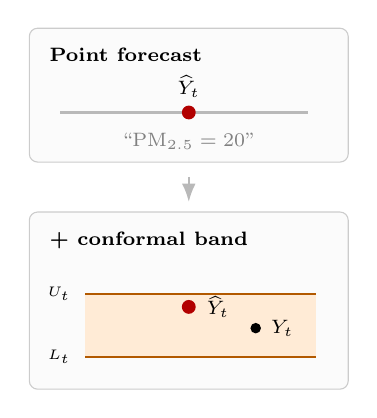
\begin{tikzpicture}[
        font=\scriptsize,
        >=Latex,
        panel/.style={draw=gray!40, rounded corners=3pt, inner sep=6pt,
                      fill=gray!3, minimum width=4.05cm}
      ]
        % ---- Panel 1: point forecast ----
        \node[panel, minimum height=1.7cm] (p1) {};
        \node[anchor=north west, font=\scriptsize\bfseries]
              at ([xshift=4pt,yshift=-4pt]p1.north west) {Point forecast};
        \draw[thick, gray!55] ([yshift=-0.22cm]p1.west) ++(0.4,0) -- ++(3.15,0);
        \coordinate (pf) at ([yshift=-0.22cm]p1.center);
        \fill[red!70!black] (pf) circle (2.5pt);
        \node[above=2pt] at (pf) {$\widehat Y_t$};
        \node[below=4pt, gray] at (pf) {``PM$_{2.5}=20$''};

        % ---- Arrow between panels ----
        \draw[-{Latex}, thick, gray!55] ([yshift=-0.18cm]p1.south) -- ++(0,-0.32);

        % ---- Panel 2: conformal band ----
        \node[panel, minimum height=2.25cm, below=0.62cm of p1] (p2) {};
        \node[anchor=north west, font=\scriptsize\bfseries]
              at ([xshift=4pt,yshift=-4pt]p2.north west) {+ conformal band};
        \fill[orange!16] ([xshift=0.72cm,yshift=-1.05cm]p2.north west)
              rectangle ([xshift=-0.42cm,yshift=0.42cm]p2.south east);
        \draw[thick, orange!70!black]
              ([xshift=0.72cm,yshift=-1.05cm]p2.north west)
              -- ([xshift=-0.42cm,yshift=-1.05cm]p2.north east);
        \draw[thick, orange!70!black]
              ([xshift=0.72cm,yshift=0.42cm]p2.south west)
              -- ([xshift=-0.42cm,yshift=0.42cm]p2.south east);
        \node[left=2pt, font=\tiny] at ([xshift=0.72cm,yshift=-1.05cm]p2.north west) {$U_t$};
        \node[left=2pt, font=\tiny] at ([xshift=0.72cm,yshift=0.42cm]p2.south west) {$L_t$};
        \coordinate (yh) at ([yshift=-0.08cm]p2.center);
        \coordinate (yt) at ([xshift=0.85cm,yshift=-0.35cm]p2.center);
        \fill[red!70!black] (yh) circle (2.5pt);
        \node[right=3pt] at (yh) {$\widehat Y_t$};
        \fill[black] (yt) circle (1.9pt);
        \node[right=2pt] at (yt) {$Y_t$};
      \end{tikzpicture}
    \end{column}
    \begin{column}{0.50\textwidth}
      {\footnotesize
      \begin{itemize}\setlength\itemsep{0.85em}
        \item \textbf{Need:} alerts need a safe range, not one risky guess.
        \item \textbf{Recipe:} use recent $|Y-\widehat Y|$ to set width ---
              large recent errors $\Rightarrow$ wider band.
        \item \textbf{No normal assumption:} AQ errors are spiky / quiet;
              conformal is distribution-free.
        \item \textbf{``95\%'':} about 95 of 100 hours, $Y_t\in[L_t,U_t]$
              (coverage).
      \end{itemize}
      }
    \end{column}
  \end{columns}
  \vspace{0.55em}
  {\footnotesize
  \centering
  From $\widehat Y_t$ alone to a band $[L_t,U_t]$ with target coverage $1-\alpha=95\%$.\par
  }
\end{frame}

\begin{frame}{Conformal formula}
  {\footnotesize
  \centering
  \renewcommand{\arraystretch}{1.35}
  \begin{tabular}{@{}r@{\hspace{0.7em}}c@{}}
    \textbf{Score}
      & $CS_t=\dfrac{|Y_t-\widehat Y_t|}{\widehat U_t}$ \\
    \textbf{Quantile}
      & $CQ_t=Q_{1-\alpha}\!\big(CS_{t-\kappa+1:t}\big)$ \\
    \textbf{Interval}
      & $PI_t=\widehat Y_t\pm CQ_t\,\widehat U_t$ \\
  \end{tabular}
  }
  \vspace{0.35em}
  {\scriptsize
  \centering
  Band edges:
  $L_t=\widehat Y_t-CQ_t\widehat U_t$,\
  $U_t=\widehat Y_t+CQ_t\widehat U_t$
  (clip $L_t\ge 0$).
  \par
  }
  \vspace{0.4em}
  \begin{columns}[T]
    \begin{column}{0.48\textwidth}
      {\footnotesize
      \begin{itemize}\setlength\itemsep{0.35em}
        \item $Y_t$, $\widehat Y_t$: truth / WaveCatBoost.
        \item $\widehat U_t$: local error scale (next slide).
        \item $CS_t$: scaled $|$error$|$ (nonconformity).
        \item $\alpha{=}0.05$ $\Rightarrow$ 95\% target.
        \item $\kappa\in\{24,168,336\}$~h (cal.\ window).
      \end{itemize}
      }
    \end{column}
    \begin{column}{0.50\textwidth}
      \begin{exampleblock}{How to use it}
        {\scriptsize
        \begin{enumerate}\setlength\itemsep{0.2em}
          \item Fit on train; residuals on a cal.\ window.
          \item Build $CS_t$; pick $\kappa$ for $\approx 95\%$ cal.\ coverage.
          \item Test: band $\widehat Y_t\pm CQ_t\widehat U_t$.
          \item Coverage $=$ share of $Y_t\in[L_t,U_t]$.
        \end{enumerate}
        }
      \end{exampleblock}
    \end{column}
  \end{columns}
\end{frame}

\begin{frame}{How $\widehat U_t$ and $CQ_t$ are computed}
  \begin{columns}[T]
    \begin{column}{0.48\textwidth}
      \begin{block}{$\widehat U_t$ --- local error scale}
        {\footnotesize
        Residual $e_t=Y_t-\widehat Y_t$.\\[0.35em]
        Default: \textbf{24-h rolling MAE}
        \[
          \widehat U_t=
          \operatorname{mean}\big(|e_{t-23}|,\ldots,|e_t|\big).
        \]
        Large recent mistakes $\Rightarrow$ large $\widehat U_t$
        $\Rightarrow$ wider band via $CQ_t\widehat U_t$.\\[0.35em]
        Multi-step test (no new $Y$ yet): freeze one robust
        $u^\star$ from calibration and reuse it.
        }
      \end{block}
    \end{column}
    \begin{column}{0.50\textwidth}
      \begin{block}{$CQ_t=Q_{1-\alpha}(CS_{t-\kappa+1:t})$}
        {\footnotesize
        \begin{enumerate}\setlength\itemsep{0.3em}
          \item Take the last $\kappa$ scores
                $CS_{t-\kappa+1},\ldots,CS_t$.
          \item Sort them.
          \item Take the $(1-\alpha)$-quantile
                ($\alpha{=}0.05$ $\Rightarrow$ $\approx$ 95th percentile).
        \end{enumerate}
        \vspace{0.25em}
        $CQ_t$ is the cutoff for a ``normal'' scaled error.\\
        Scores with $CS\le CQ_t$ fall inside
        $\widehat Y_t\pm CQ_t\widehat U_t$.
        }
      \end{block}
    \end{column}
  \end{columns}
\end{frame}

\begin{frame}{Do the intervals work? (7-day test)}
  {\footnotesize
  \textbf{Purpose:} letter-style 7-day PM$_{2.5}$ band --- does truth sit inside the
  95\% window around WaveCatBoost?
  }
  \vspace{0.3em}
  \centering
  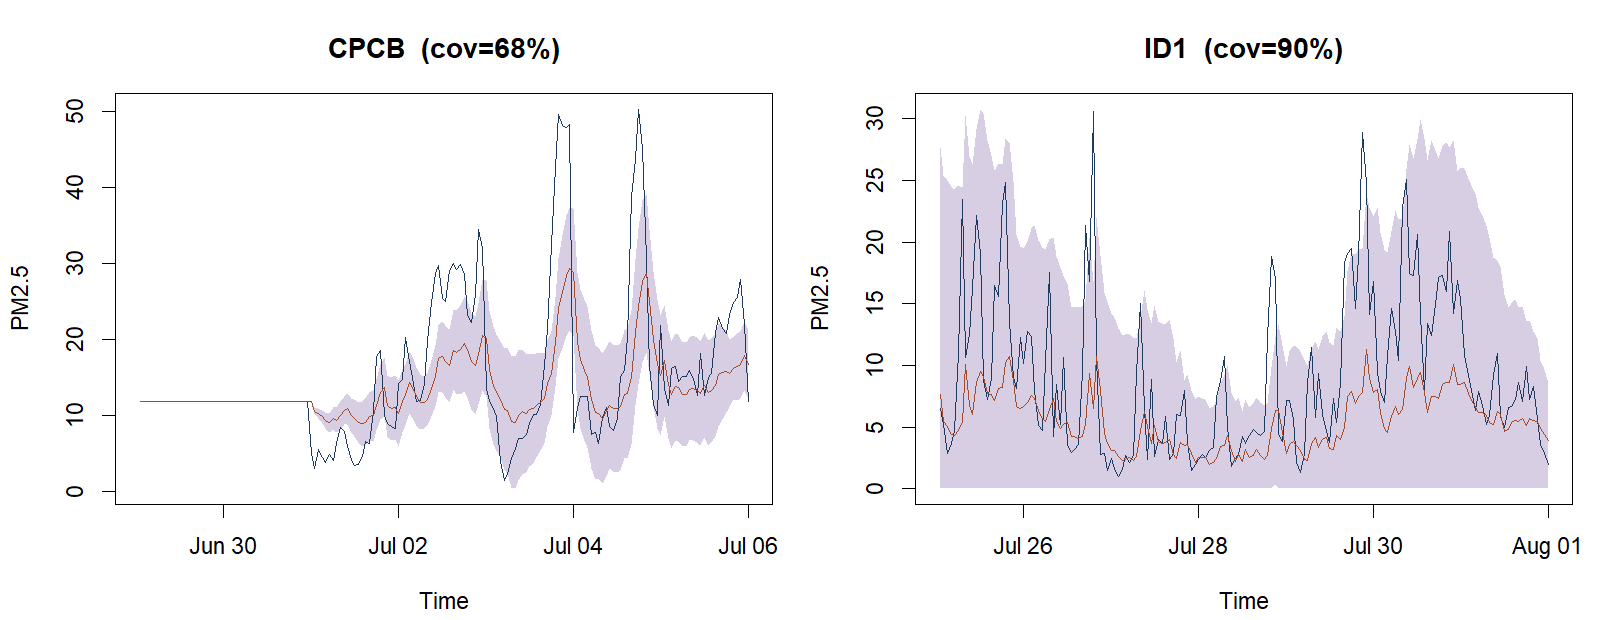
\includegraphics[width=0.98\linewidth,height=0.52\textheight,keepaspectratio]{conformal_cpcb_id1.png}
  \vspace{0.15em}
  {\footnotesize
  \begin{itemize}\setlength\itemsep{0.12em}
    \item \textbf{Black} $=$ actual;\ \textbf{orange} $=$ WaveCatBoost;\
          \textbf{shaded} $=$ 95\% residual PI $[L_t,U_t]$
          (same colours as Rmd §8.2).
    \item Paper residual PI on this window: CPCB / ID1 coverage $\approx 95\%$
          (widths $\approx 12.0$ / $11.7$).
  \end{itemize}
  }
\end{frame}

\begin{frame}{7-day paper residual PI --- summary}
  {\footnotesize
  \centering
  \begin{tabular}{lccc}
    \toprule
    Sensor & Coverage & Mean width & Point MAE \\
    \midrule
    CPCB     & 0.95 & 12.0 & 1.48 \\
    ID1      & 0.95 & 11.7 & 1.96 \\
    Shillong & 0.95 & 19.3 & 3.56 \\
    \bottomrule
  \end{tabular}
  }
  \vspace{0.7em}
  \begin{exampleblock}{Protocol}
    Rolling 1-step WaveCatBoost (letter notebook) + 95\% quantile of
    $|Y-\widehat Y|$ on the plotted 7-day window ($\alpha=0.05$).
  \end{exampleblock}
\end{frame}


\section{Experimental Results}
% Experimental results frames moved into segments/4_conclude.tex
% (Error metrics + recursive bake-off now sit before conformal).


\section{Wrap-up}
\begin{frame}{Summary}
  \begin{itemize}
    \item WaveCatBoost $=$ Haar MODWT $+$ CatBoost per band $+$ reconstruct.
    \item Haar remains a strong default vs D4/LA8.
    \item Conformal bands add uncertainty; CQR improves coverage / width where split conformal struggles.
    \item \textbf{Recursive bake-off:} wavelet helps vs raw trees on several cells.
    \item \textbf{1-step vs Table~1:} same ranking (WaveCB wins); our MASE is lower, but
          absolute digits are not a fair ``we beat the paper'' claim --- compare ranks/gaps.
  \end{itemize}
\end{frame}


\section*{References}
\begin{frame}[allowframebreaks]
  \frametitle{References}
  \bibliographystyle{ieeetr}
  \bibliography{ref.bib}
\end{frame}

\end{document}
